\section{Physical Design}

Here we will discuss the physical design of the system, so the creation of indexes


\subsection{Indexes for operations}

\subsubsection{Operation1} 


\paragraph{Explain Plan} \leavevmode \newline

\begin{figure}[H]
    \centering
    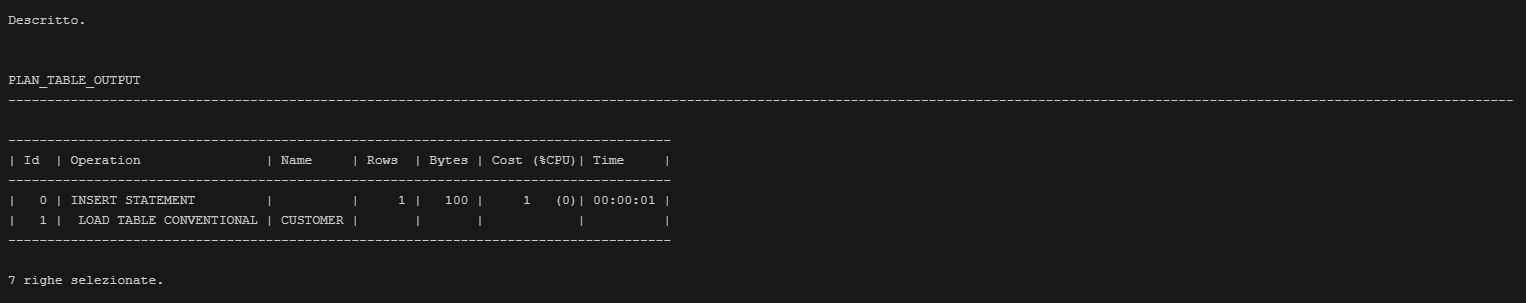
\includegraphics[width=\textwidth]{images/ExPlan1.png}
    \caption{Operation1}
\end{figure}


\paragraph{Auto-Trace} \leavevmode \newline
\begin{figure}[H]
    \centering
    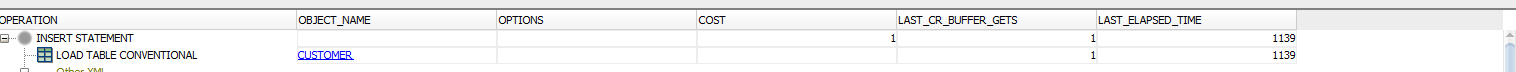
\includegraphics[width=\textwidth]{images/Op1Index.png}
    \caption{Operation1}
\end{figure}

Since the operation is a simple insert, it doesn't require any indexes to be created. The data will be inserted into the table as it is.

\subsubsection{Operation2}

\paragraph{Explain Plan} \leavevmode \newline

\begin{figure}[H]
    \centering
    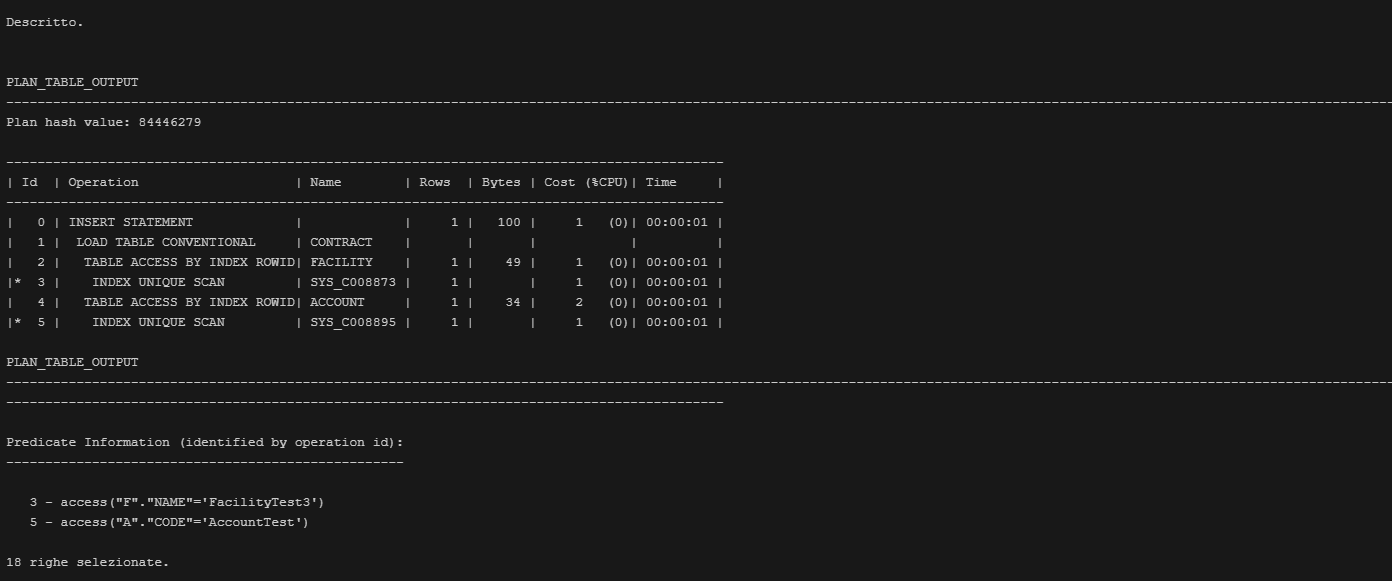
\includegraphics[width=\textwidth]{images/ExPlan2.png}
    \caption{Operation2}
\end{figure}

\paragraph{Auto-Trace} \leavevmode \newline

\begin{figure}[H]
    \centering
    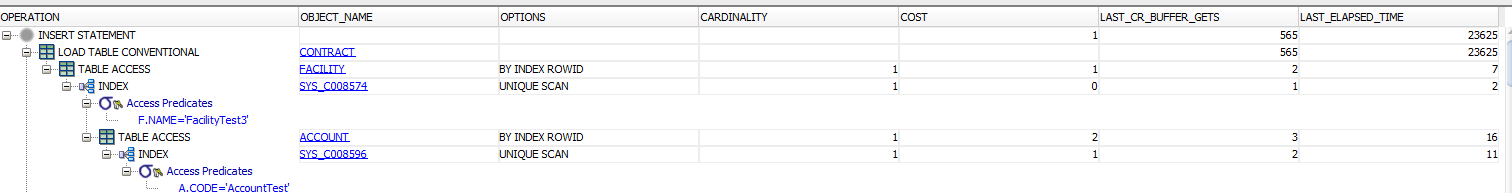
\includegraphics[width=\textwidth]{images/Op2Index.png}
    \caption{Operation2}
\end{figure}

Since the operation is a simple insert, it doesn't require any indexes to be created. The data will be inserted into the table as it is.

\subsubsection{Operation3}
The operation is an update, so the creation of an index is not required. However, we check for the existence of the Facility and of the Team but they are primary keys, so they are already indexed.

\paragraph{Explain Plan} \leavevmode \newline

\begin{figure}[H]
    \centering
    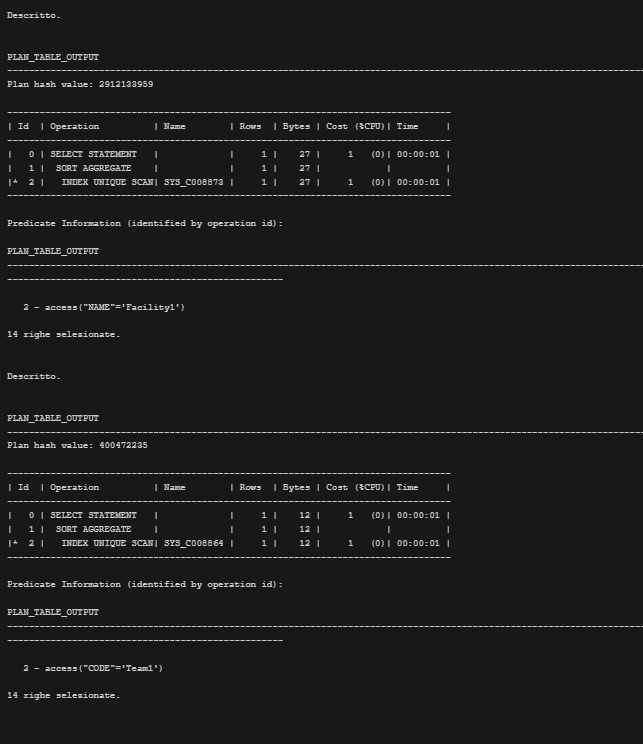
\includegraphics[width=\textwidth]{images/ExPlan3.png}
    \caption{Operation3}
\end{figure}

\paragraph{Auto-Trace} \leavevmode \newline

\begin{figure}[H]
    \centering
    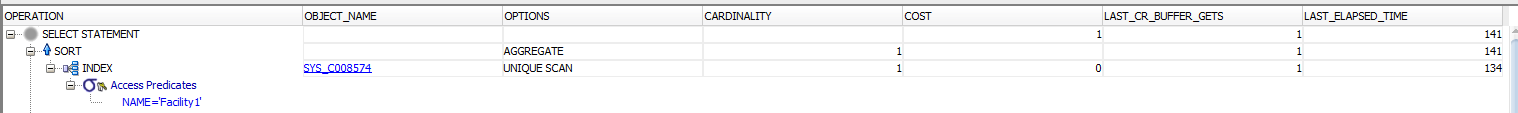
\includegraphics[width=\textwidth]{images/FacilityName.png}
    \caption{Facility Name Index}
\end{figure}

\begin{figure}[H]
    \centering
    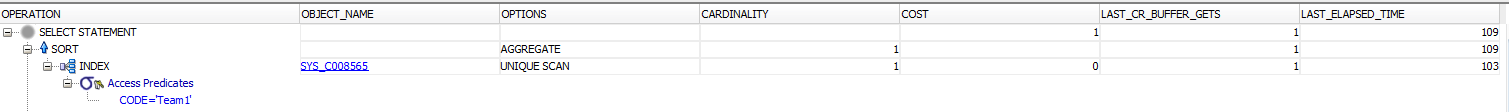
\includegraphics[width=\textwidth]{images/TeamCode.png}
    \caption{Team Code Index}
\end{figure}

\subsubsection{Operation4}

The first part is the selection of the oldest employee who is a manager. We can create an index on the Date of Birth (DoB) attribute of the Employee table, so that they will be ordered by DoB and we can fetch the first row.

\paragraph{Explain Plan} \leavevmode \newline

\begin{figure}[H]
    \centering
    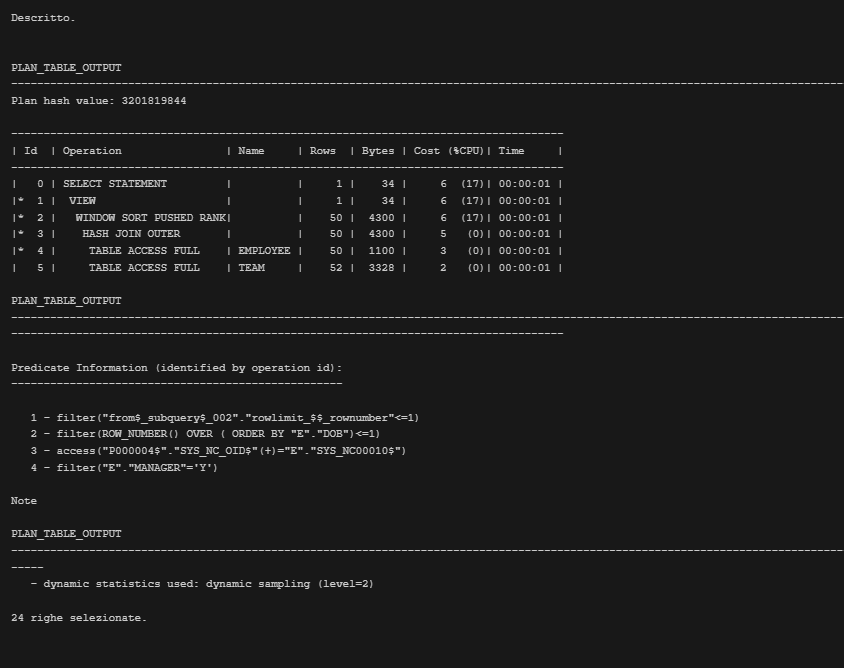
\includegraphics[width=\textwidth]{images/ExPlan4.png}
    \caption{Operation4}
\end{figure}

\paragraph{Auto-Trace} \leavevmode \newline

\begin{figure}[H]
    \centering
    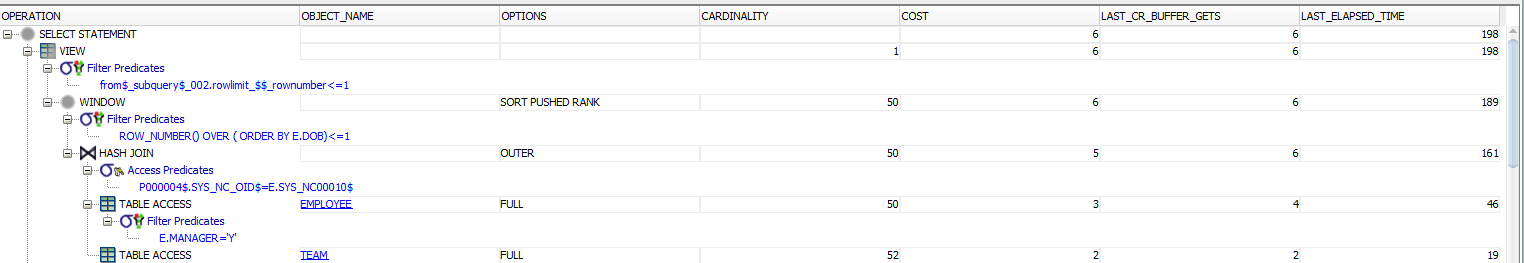
\includegraphics[width=\textwidth]{images/OldManNOIndex.png}
    \caption{Autotrace without Index}
\end{figure}

By using the autotrace we can see that here we are not using any index. Let's create the index

\begin{lstlisting}
    CREATE INDEX Employee_DoB_Index ON Employee(DoB);
\end{lstlisting}

\begin{figure}[H]
    \centering
    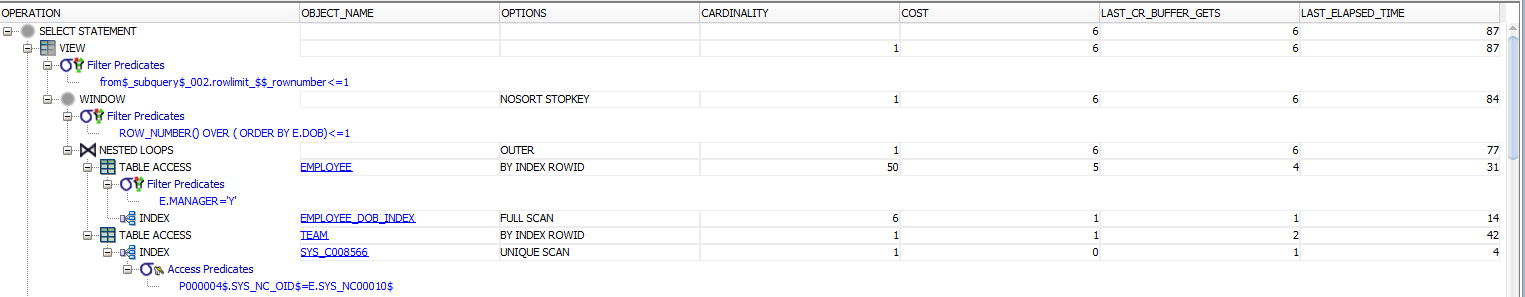
\includegraphics[width=\textwidth]{images/OldManWithIndex.png}
    \caption{Autotrace with Index}
\end{figure}

We can see that now we are using the Employee\_DoB\_Index index to fetch the first row (the Autotrace shows UNIQUE SCAN). The second part of the operation is a simple sselection. It uses Facility.Name with is already indexed.

\subsubsection{Operation5}


Operation five is a selection sorted by FacilityEfficiency. However, even with an index on that attribute, the Autotrace shows that the index is not used.

\paragraph{Explain Plan} \leavevmode \newline

\begin{figure}[H]
    \centering
    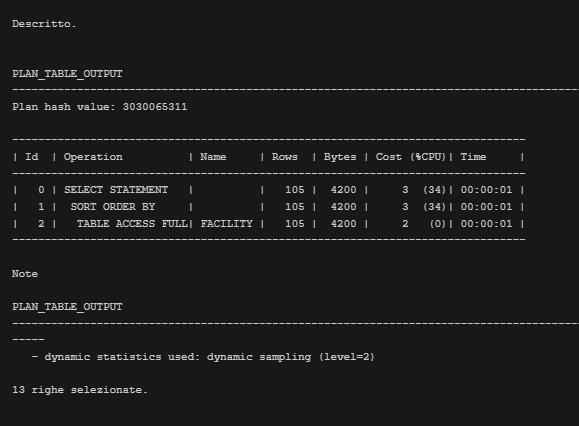
\includegraphics[width=\textwidth]{images/ExPlan5.png}
    \caption{Operation5}
\end{figure}

\paragraph{Auto-Trace} \leavevmode \newline

\begin{figure}[H]
    \centering
    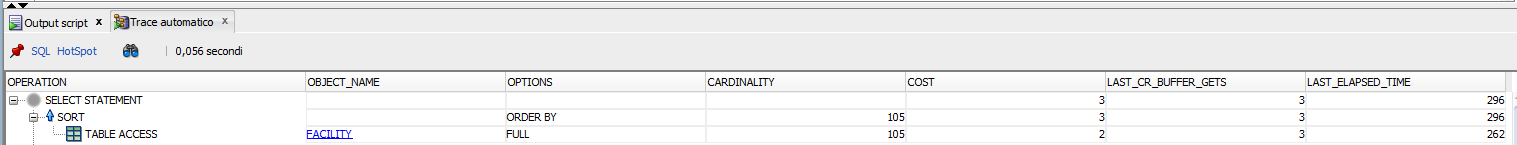
\includegraphics[width=\textwidth]{images/EffScore.png}
    \caption{Autotrace}
\end{figure}